\documentclass[9pt,conference]{IEEEtran}
\usepackage[utf8]{inputenc}
\usepackage[brazil]{babel}

% Diversos
\usepackage{csquotes}
\usepackage{graphicx}
\usepackage{verbatim}
\usepackage{hyperref}
\usepackage{smartdiagram}

% Título
\title{Utilizando Redes Convolucionais de Grafos Espaço-Temporais para o Reconhecimento da Línguas de Sinais}
%\author{Cleison Correia de Amorim}
\date{Outubro 2018}

\author{
    \IEEEauthorblockN{Cleison Correia de Amorim}
    \IEEEauthorblockA{Centro de Informática\\
    Universidade Federal de Pernambuco\\
    Email: cca5@cin.ufpe.br}
}

% Comandos
% 'image': definição de imagem
\newcommand{\image}[4][\linewidth] {
    \begin{figure}[ht]
    \centering
    \includegraphics[width=#1]{#3}
    \caption{#4}
    \label{#2}
    \end{figure}
}

% 'refimage': referências de imagens
\newcommand{\refimage}[1] {figura \ref{#1}}

% 'refsection': referências de seções
\newcommand{\refsect}[1] {seção "\nameref{#1}"}

\begin{document}
\maketitle
\begin{abstract}
Este projeto propõe a aplicação de técnicas de \textit{deep learning} para a transcrição das características fonológicas da língua de sinais para o modelo computacional CORE-SL proposto por \cite{antunes-2015}. 

[adicionar abstract ...]
\end{abstract}
%\begin{IEEEkeywords}
%Broad band networks, quality of service, WDM.
%\end{IEEEkeywords}


\section{Introdução}
\label{sec:introducao}
Pode-se observar um número considerável de estudos que propõem-se a realizar a tradução de diferentes línguas de sinais para a língua falada correspondente. Entretanto, muito desses estudos ficam limitados frente ao contexto cotidiano do Surdo por desconsiderarem aspectos relevantes da fonologia da língua como os movimentos, expressões não-manuais, locação e orientação das mãos do interlocutor \cite{quadros-2004}. É comum também que tais estudos restrinjam seu campo de atuação ao âmbito da datilologia\footnote{
Datilologia – também conhecida como alfabeto digital ou alfabeto manual, consiste na soletração manual de palavras pelos Surdos. É geralmente utilizada para introduzir uma palavra que ainda não possui um sinal equivalente \cite{quadros-2004}\cite{pereira-choi-2011}.
}, que na prática é aplicada apenas em contexto restritos da comunicação desses indivíduos.

Em \cite{antunes-hcisl-2011}, os autores apresentam outros fatores que justificam a limitação em trazer muitos desses estudos para a realidade do Surdo: 
\begin{enumerate}
    \item O uso de equipamentos como luvas, acelerômetros e outros sensores que são de difícil acesso; 
    \item A adoção de métodos e tecnologias que não empatizam com a realidade surdo, restringindo sua movimentação ou deixando de considerar aspectos importantes, como as expressões faciais;
    \item O uso de métodos que mapeiam sinais diretamente para palavras, e que tornam-se facilmente obsoletos mediante a introdução de novos sinais ou quando confrontados com variações linguísticas como gírias e regionalismos; 
    \item A utilização de imagens estáticas para o treinamento de modelos, que desconsideram a dinâmica da língua.
\end{enumerate}

Diante dessas limitações, foi introduzido em \cite{antunes-hcisl-2011} a proposta de uma arquitetura capaz de considerar os aspectos fonológicos da língua e de viabilizar a interação homem-máquina por meio dos sinais, a qual foi denominada HCI-SL. A \refimage{fig:hcisl} apresenta essa arquitetura, onde uma API interna compreendendo tecnologias de visão computacional e processamento de linguagem natural proveem uma interface padrão para ferramentas e serviços externos como dicionários, tradutores e aplicações de finalidades diversas.

\image
	[5cm]
    {fig:hcisl}
    {images/hcisl}
    {Arquitetura HCI-SL apresentada por \cite{antunes-hcisl-2011}.}

Para a arquitetura acima funcionar, foi necessário primeiro definir o CORE-SL, que consiste num modelo computacional para descrição dos sinais e suas características fonológicas. Ele estabelece um padrão de representação a ser adotado pelas peças que compõem a arquitetura HCI-SL e pelas aplicações e serviços desenvolvidos a partir dela.

De acordo com os autores, o CORE-SL:

\begin{quote}
[...] agrega flexibilidade e um nível de detalhamento capazes de proporcionar alternativas para um tratamento computacional robusto e para auxiliar às diferentes necessidades de aplicação. Este modelo atuará como um dos pilares de sustentação na construção de artefatos tecnológicos que considerem as necessidades deste perfil de usuário e tornem a comunicação usuário-sistema natural para ele. \cite{antunes-2011}
\end{quote}

 A \refimage{fig:coresl-interfaces} ilustra as interações do CORE-SL com um conjunto de serviços idealizados ou em desenvolvimento por pesquisadores da Universidade Federal do Paraná - UFPR. Nela, o modelo exerce um papel central para a comunicação das peças envolvidas.

\image
    {fig:coresl-interfaces}
    {images/coresl_interfaces}
    {CORE-SL como peça chave para a comunicação de outros serviços}

A \refimage{fig:coresl-sinalarvore} mostra um exemplo de descrição do sinal árvore através do modelo CORE-SL.

\image
    {fig:coresl-sinalarvore}
    {images/sinal_arvore}
    {Representação do sinal árvore escrito segundo o CORE-SL}
    

\section{Redes Convolucionais de Grafos Espaço-Temporais}

Será utilizado para este trabalho o modelo \textit{Spatial-Temporal Graph Convolutional Networks} (ou Redes Neurais de Grafos Espaço-Temporais) apresentado por \cite{st-gcn-2018}, devido à sua capacidade de lidar com o movimento humano sob duas perspectivas distintas. 

(e também da língua de sinais), como a sua articulação dentro do espaço e no decorrer do tempo.

\image
	[4cm]
    {fig:st-gcn-graph}
    {images/st_gcn_graph}
    {Grafo espaço-temporal de uma sequência de esqueletos utilizados pelo ST-GCN, onde os pontos azuis denotam as juntas do corpo. Os vértices intra-corporais são definidos com base nas conexões naturais do corpo humano. Os vértices inter-frames, por sua vez, conectam as mesmas juntas entre frames consecutivos para denotar seu movimento no decorrer do tempo \cite{st-gcn-2018}.}


Adicionalmente, tem-se como estratégia utilizar a biblioteca OpenPose para extrair os pontos do corpo dos atores presentes no \textit{dataset} acima e produzir uma entrada potencialmente mais rica para o modelo. A OpenPose é capaz de detectar os atores e fornecer cerca de 135 pontos referentes a partes de seus corpos, como mãos, braços e rosto, conforme descrito em \cite{cao-realtime-2017}, \cite{simon-hand-2017}, \cite{wei-cpm-2016} e no endereço \url{https://github.com/CMU-Perceptual-Computing-Lab/openpose}. Apesar disso, o acesso à quantidade considerável de recursos computacionais requeridos por essa biblioteca durante a execução do projeto (como por exemplo, GPUs com mais de 4GB de memória), pode ser um fator limitador em potencial para sua aplicação neste momento.

\image
	[4cm]
    {fig:keypoints-pose}
    {images/keypoints_pose_COCO_18}
    {Representação dos 18 pontos do corpo extraídos pelo OpenPose e utilizados pelo modelo ST-GCN.}


\section{Dataset}
\label{sec:dados-utilizados}
Será utilizado o \textit{dataset} \textit{American Sign Language Lexicon Video Dataset} (ASLLVD)\footnote{\textit{American Sign Language Lexicon Video Dataset} (ASLLVD) - disponível no endereço \url{http://vlm1.uta.edu/~athitsos/asl_lexicon/}}, que é composto por vídeos de sinais realizados por diferentes atores, com diferentes níveis de fluência na língua de sinais. O \textit{dataset} também contém arquivos de metadados que determinam o nome e os respectivos \textit{frames} de início e fim para os sinais nos vídeos gravados. Ele é apresentado em mais detalhes em \cite{athitsos-asldataset-2008}.

\image
    {fig:asllvd-example}
    {images/asllvd_example}
    {Exemplo de representação do sinal \textit{"MERRY-GO-ROUND"} capturado em três perspectivas distintas no \textit{dataset} ASLLVD \cite{athitsos-asldataset-2008}.}

Para que os vídeos possam ser utilizados como entrada para o modelo ST-GCN, é necessário antes realizar um pré-processamento consistindo nas seguintes etapas:
\begin{enumerate}
    \item Segmentar vídeos: as amostras do  ASLLVD compreendem seções onde foram gravados vários sinais em sequência. Devido a isso, é necessário segmentá-los em vários vídeos contendo sinais individuais, utilizando para isso os arquivos de metadados disponibilizados com o \textit{dataset}, que indicam os momentos de início e término de cada sinal;
    \item Aumentar \textit{dataset}: foi observado no \textit{dataset} acima que não há um grande número de variações para os sinais contidos. Existe geralmente 1 ou 2 vídeos por sinal e, para melhorar o desempenho do modelo, será necessário gerar variações a partir dos vídeos existentes;
    \item Estimar pose: em seguida, é necessário extrair os pontos do corpo dos atores para cada frame dos vídeos, através da biblioteca OpenPose para em seguida agrupá-los em um único arquivo JSON. Para o propósito deste projeto serão considerados 130 pontos, ou seja, além dos 18 pontos referentes ao corpo estão inclusos também os 70 pontos da face e 21 pontos para cada uma das mãos, conforme ilustrado na \refimage{fig:keypoints-face-hand};
    \item Preencher frames vazios: todas as amostras utilizadas na entrada do modelo devem possuir tamanho uniforme, conforme descrito em \cite{st-gcn-2018}. Para isso, os autores sugerem que a sequência de frames dos vídeos seja repetida até completar o tamanho de entrada, que para este trabalho será de 10 segundos (ou 30es, considerando a taxa de 30 fps);
    \item Dividir grupos de amostras: separar as amostras pré-processadas entre os grupos treinamento e validação, com uma proporção de 80\% e 20\%, respectivamente;
    \item Serializar amostras: a implementação do ST-GCN utiliza como entradas listas de objetos do Python serializados e gravados como arquivos \textit{.pkl} em disco. Sendo assim, esse processo deve ser aplicado aos conjuntos de amostras divididos no passo anterior.
\end{enumerate}

\begin{figure}[ht]
    \centering
    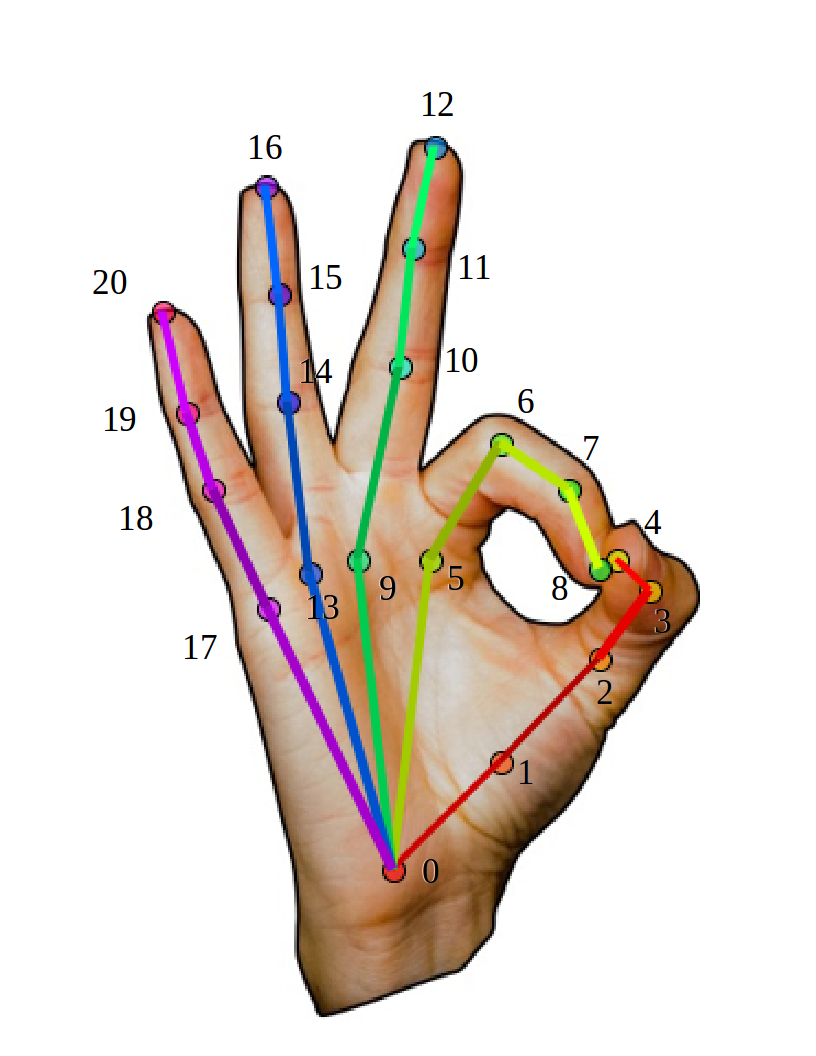
\includegraphics[width=3cm]{images/keypoints_hand}
    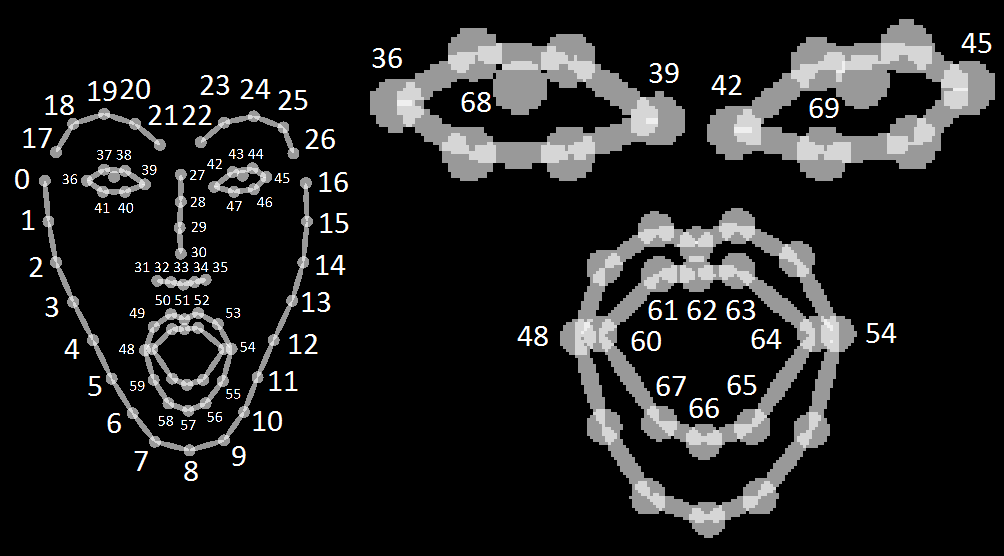
\includegraphics[width=5cm]{images/keypoints_face}
    \caption{Representação dos 21 pontos da mão e 70 pontos da face extraídos pelo OpenPose e que serão utilizados neste trabalho.}
    \label{fig:keypoints-face-hand}
\end{figure}
Como os sinais contidos no \textit{dataset} não possuem sua descrição em CORE-SL, será necessário produzir as respectivas \textit{labels} nesse formato. Entretanto, o tempo limitado para execução deste trabalho, atua como limitador na produção dessas \textit{labels} e quantidade de amostras classificadas dessa forma que será possível obter a tempo de aplicar ao modelo e extrair resultados. Uma das estratégias para lidar com isso é selecionar um conjunto de cerca das 20 características mais relevantes do CORE-SL para classificar os vídeos no primeiro momento. O CORE-SL possui um total de 100 características.


\section{Avaliação dos resultados}
Devido à restrição no número de amostras com \textit{labels} em CORE-SL que serão geradas (conforme \refsect{sec:dados-utilizados}), a estratégia inicial para validação do modelo consiste em utilizar de técnicas de validação cruzada como o K-Fold, pela sua capacidade de maximizar o uso dos dados disponíveis através de diferentes combinações entre eles.

Com relação às métricas a serem adotadas, ainda há necessidade de pesquisa quanto àquelas mais apropriadas ao tipo de modelo RNN e, principalmente, ao tipo de problema proposto acima. Apesar disso, sabe-se de antemão que essas métricas devem ser capazes de mensurar o grau de similaridade (ou proporção do acerto/erro) das saídas produzidas pelo modelo, dado que um \textit{label} em CORE-SL consiste em um XML contendo diversas características fonológicas que permitem um julgamento do tipo "quão correta está a descrição do sinal produzida pelo modelo", "quantas das características estão corretas?" ou "o XML obtido está 90\% semelhante com relação ao XML de referência". Métricas que limitem a avaliação de uma forma binária como "certo" ou "errado" não se mostram adequadas para este problema.


% Bibliografia
\bibliographystyle{IEEEtran}
\bibliography{IEEEabrv,references.bib}

\end{document}
%%